\chapter{Introducción Específica} % Main chapter title

\label{Chapter2}

%----------------------------------------------------------------------------------------
%	SECTION 1
%----------------------------------------------------------------------------------------

Este capítulo provee una introducción más detallada de todo el trabajo realizado.
Se presenta al lector una explicacion del funcionamiento  de los semaforos vehiculares, una vista general del sistema, requerimientos y una explicación de las tecnologías involucradas en el desarrollo.

\section{Funcionamiento de los semaforos}

Los semáforos, también conocidos técnicamente como señales de control de tráfico, son dispositivos de señales que se sitúan en intersecciones viales y otros lugares para regular el tráfico, y por ende, el tránsito peatonal \citep{semaforo}.

Los semáforos se dividen en tres clases, que son: 

\begin{itemize}
\item Vehicular: Tiene por objeto regular el tránsito de vehículos en las intersecciones. Está compuesto esencialmente por tres faros programados para que proyecten durante un tiempo determinado un haz de luz de colores verde, amarillo y rojo.
\item Peatonal: Se hallan instalados en combinación con los vehiculares y tienen por objeto regular el paso de los peatones en intersecciones con alto volumen de tráfico.
\item Direccional: Tiene como fin informar mediante flechas, el momento adecuado para girar. 
\end{itemize}

En cuanto al funcionamiento del semaforo vehicular se puede decir que, cuando la luz es verde, significa que hay vía libre y se puede pasar. La luz amarilla advierte al conductor que se aproxima un cambio de luz. Al ver la luz roja se debe detener el auto, pues otro flujo de vehículos se interceptará en la dirección de su marcha.

En los semáforos peatonales, el significado es el siguiente: la silueta roja indica que el peatón no debe cruzar la calle, mientras que la silueta verde lo permite.

\subsection{Secuencia}
En base a la observacion del funcionamiento de los semaforos vehiculares en distintas provincias de la Republica Argentina como ser Córdoba, Catamarca y Tucumán se detecto las siguientes secuencias:

\begin{itemize}
\item Rojo, Rojo-Amarillo , Verde, Amarillo y Rojo
\item Rojo, Amarillo, Verde, Amarillo y Rojo
\item Rojo, Amarillo y Verde
\end{itemize}

\section{Esquema general del sistema}
 En la  siguiente figura \ref{fig:diagramaGeneral} se observa  el sistema en una  version simplificada
\begin{figure}[h]
	\centering
	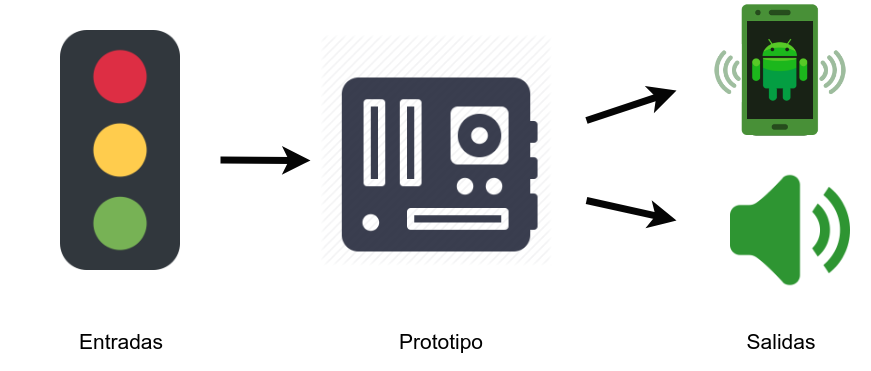
\includegraphics[scale=.4]{./Figures/diagramaGeneral.png}
	\caption{El lector no sabe por qué de pronto aparece esta figura.}
	\label{fig:questionMark}
\end{figure}

\section{Requerimientos}

\section{Tecnologias de comunicacion}